\documentclass[tikz]{standalone}
\usepackage{pgfplots}
\pgfplotsset{compat=1.15}
\usepackage{mathrsfs}
\usetikzlibrary{arrows,calc}
\usepackage{tkz-euclide}
\pagestyle{empty}

\definecolor{AngleClr}{rgb}{0,0.39215686274509803,0}
\definecolor{ShapeClr}{rgb}{0.6,0.2,0}
\definecolor{BlueClr}{RGB}{108, 166, 224}


\begin{document}

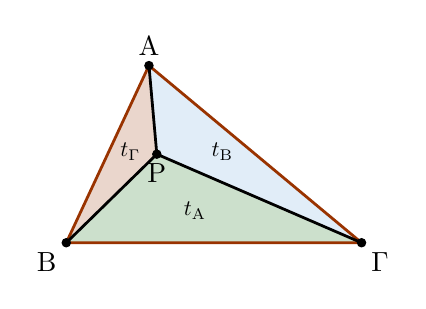
\begin{tikzpicture}[scale=.75]
\tkzSetUpLine[line width=1pt,color=black]
\tkzSetUpPoint[fill=black]

\tkzDefPoints{0/0/B,1.4/3/A,5/0/C}

\tkzDefBarycentricPoint(A=3,B=2,C=1) \tkzGetPoint{P}

\tkzDefMidPoint(B,C) \tkzGetPoint{MA}
\tkzDefMidPoint(A,C) \tkzGetPoint{MB}
\tkzDefMidPoint(A,B) \tkzGetPoint{MC}

\tkzFillPolygon[fill=white](A,B,C)

\tkzInterLL(B,MB)(C,MC)
\tkzGetPoint{G}

\tkzFillPolygon[fill=ShapeClr,fill opacity=0.2](A,B,P)
\tkzFillPolygon[fill=AngleClr,fill opacity=0.2](B,C,P)
\tkzFillPolygon[fill=BlueClr,fill opacity=0.2](C,A,P)

\tkzDrawPolygon[color=ShapeClr](A,B,C)
\tkzDrawPoints[size=3](A,B,C,P)
\tkzDrawSegments[color=black](P,A P,B P,C)

\tkzLabelPoint[above](A){$\rm A$}
\tkzLabelPoint[below left](B){$\rm B$}
\tkzLabelPoint[below right](C){$\rm \Gamma$}
\tkzLabelPoint[below](P){$\rm P$}

\tkzDefTriangleCenter[centroid](B,C,P) \tkzGetPoint{GA}
\tkzDefTriangleCenter[centroid](C,A,P) \tkzGetPoint{GB}
\tkzDefTriangleCenter[centroid](A,B,P) \tkzGetPoint{GC}

\tkzLabelPoint[scale=0.8,yshift=0.3cm](GA){$t_{\rm A}$}
\tkzLabelPoint[scale=0.8,yshift=0.3cm](GB){$t_{\rm B}$}
\tkzLabelPoint[scale=0.8,yshift=0.3cm,xshift=0.1cm](GC){$t_{\rm \Gamma}$}

\end{tikzpicture}

\end{document}
